\section{Integrated Circuit ADC/DAC}
\subsection{High Voltage, Low Frequency}
Also included in the lab instructions was a schematic for a combined ADC/DAC
circuit in which the outputs of an analog to digital converter is fed
immediately into the inputs of a digital to analog converter.  This allows
students to observe the overall accuracy of the ADC and DAC when pipelined, as
well as observing how well the system reproduces an arbitrary input.  A PSpice
capture of this schematic is shown in Figure~\ref{f:combined_schem}.
%
\begin{figure}[H]
\centering
	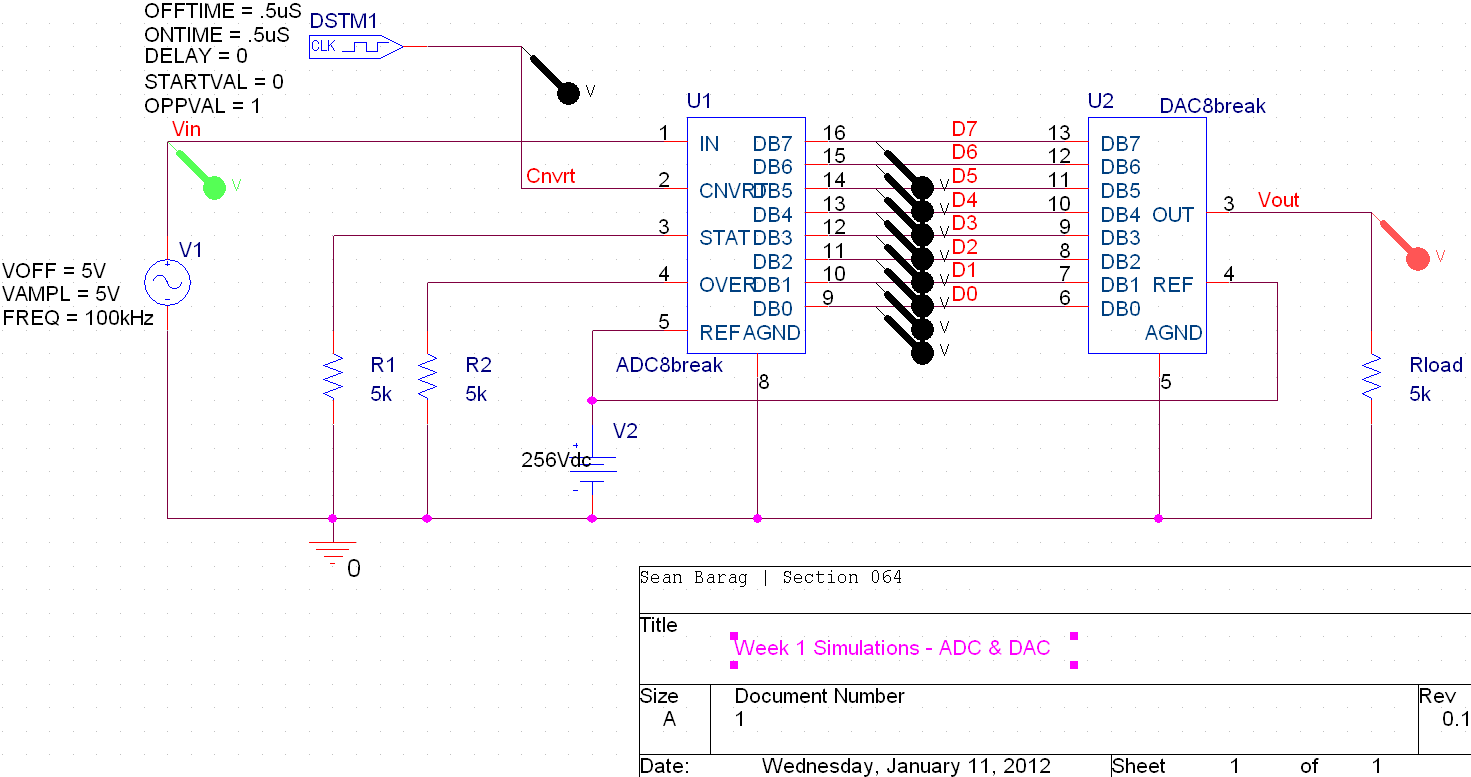
\includegraphics[width=.8\textwidth]{img/shot/part3_schem_cropped.PNG}
	\parbox{.8\textwidth}{
	\caption[Integrated Circuit --- Schematic]{Instructor provided schematic
	for the integrated circuit ADC/DAC.  Note that there are absolutely no
	elements between the outputs of the ADC and the inputs of the DAC.  This
	represents an idealized case that is not relevant in the final voice
	recorder design.}
	\label{f:combined_schem}}
\end{figure}
%
The circuit was simulated using a transient analysis
over~\SI{20}{\micro\second}, allowing the sinusoidal input to complete two full
periods.  After the simulation completed, PSpice produced the plot in
Figure~\ref{f:combined_plot1}.
%
\begin{figure}[H]
\centering
	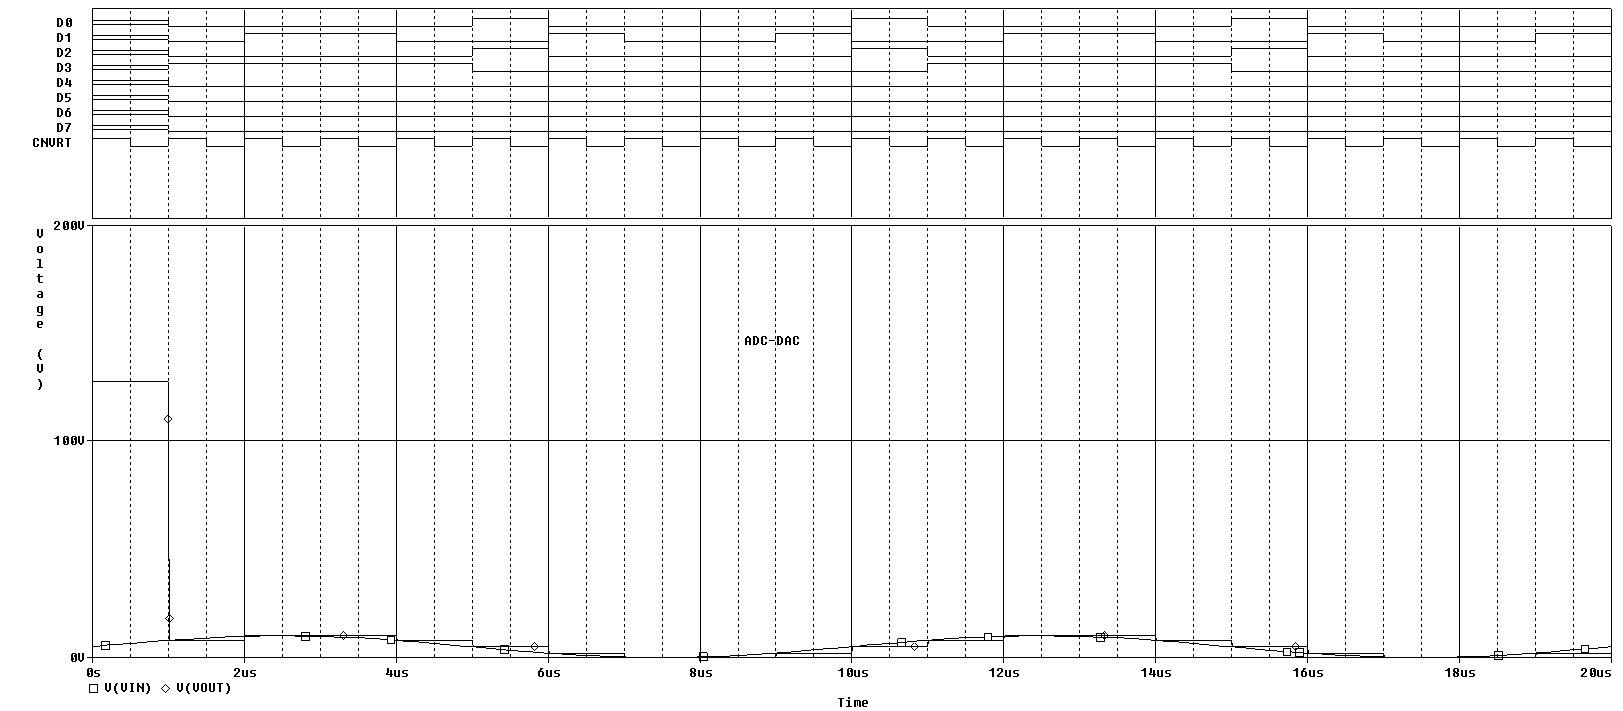
\includegraphics[width=.8\textwidth]{img/plot/part3_plot1.PNG}
	\parbox{.8\textwidth}{
	\caption[Integrated Circuit --- Initial Results]{PSpice-generated plot of
	the initially simulated integrated circuit (IC) ADC/DAC.}
	\label{f:combined_plot1}}
\end{figure}
%
Note that the time resolution of the system's output is dependant on the clock
frequency provided to the ADC.  In this configuration, the output can only
change once every microsecond.

\subsection{Low Voltage, High Frequency}
The output voltage of the DAC is determined by an equation very similar
to~\eqref{eq:dac}, as shown in~\eqref{eq:dac_ic}.
%
\begin{equation}
	V_\text{out} = V_\text{ref} \left[
		\frac{D_0}{256} +
		\frac{D_1}{128} +
		\frac{D_2}{64}  +
		\frac{D_3}{32}  +
		\frac{D_4}{16}  +
		\frac{D_5}{8}   +
		\frac{D_6}{4}   +
		\frac{D_7}{2} \right]
	\label{eq:dac_ic}
\end{equation}
%
In the case of a full-scale input to the DAC of~$11111111_2$, the output in
this configuration would be
%
\begin{equation*}
	\SI{256}{\volt} \cdot \frac{255}{256} = \SI{255}{\volt} \qquad \text{,}
\end{equation*}
%
a value that is far too large to be safely used for small
scale audio applications.  The reference voltage for the system was tuned
using~\eqref{eq:dac_ic} so that the full scale output of the DAC would be
roughly~\SI{10}{\volt}.  This resulted in a calculated reference voltage
of~\SI{10.0392157}{\volt}.  The clock frequency was also increased
from~\SI{1}{\mega\hertz} to~\SI{10}{\mega\hertz} as per the lab instructions.

Once the system was reconfigured, the~\SI{20}{\micro\second} transient analysis
was repeated, producing the plot in Figure~\ref{f:combined_plot2}.
%
\begin{figure}[H]
\centering
	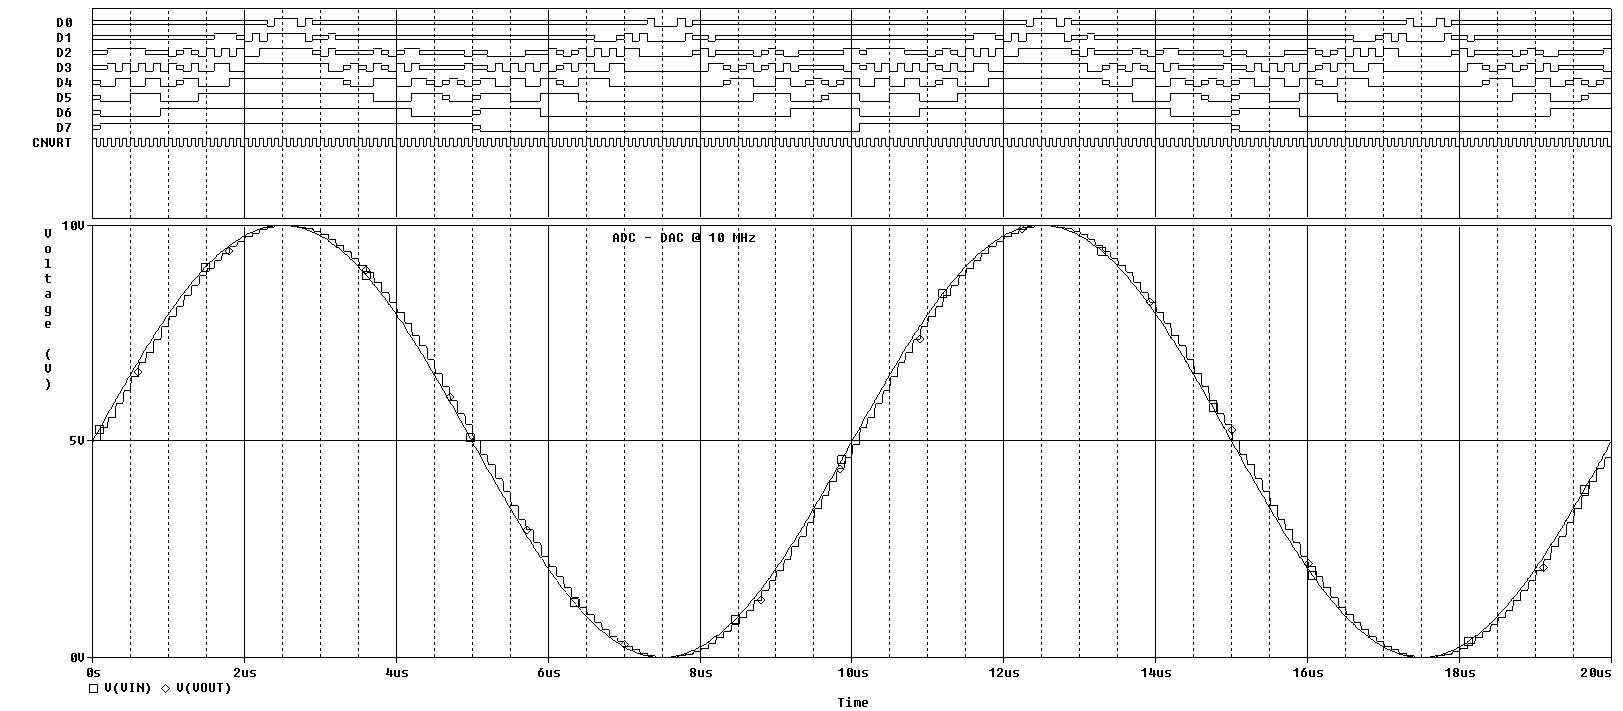
\includegraphics[width=.8\textwidth]{img/plot/part3_plot2.PNG}
	\parbox{.8\textwidth}{
	\caption[Integrated Circuit --- Tuned Results]{Plot of the tuned IC ADC/DAC
	as simulated by Cadence PSpice.  Note that the output is now limited
	to~\SI{10}{\volt} maximum, as compared to the high-voltage system shown in
	Figure~\ref{f:combined_plot1}.}
	\label{f:combined_plot2}}
\end{figure}
%
As with the high-voltage configuration, the system's time resolution is
dependant on the clock frequency feeding the ADC.  For the reconfigured system,
the time resolution is just~\SI{100}{\nano\second}.  This is evident in
Figure~\ref{f:combined_plot2}, as the output waveform more closely matches the
input than in the high-voltage case.
